% \section{Bài toán Điều khiển Tối ưu (Optimal Control Problem - OCP)}
% \label{sec:ocp}

% Bài toán điều khiển tối ưu (OCP) đóng vai trò cốt lõi trong việc tìm kiếm quỹ đạo và tín hiệu điều khiển tốt nhất cho các hệ thống động lực học sao cho tối thiểu hóa một hàm chi phí, đồng thời thỏa mãn các ràng buộc về động lực học, trạng thái và tín hiệu điều khiển.

% Dạng tổng quát của bài toán OCP thời gian liên tục được phát biểu như sau:
% \begin{align}
%     \min_{x(\cdot), u(\cdot)} \quad & \int_{t_0}^{t_f} L(x(t), u(t)) \, dt + E(x(t_f)) \label{eq:ocp_objective} \\
%     \text{subject to:} \quad & \dot{x}(t) = f(x(t), u(t)), \quad t \in [t_0, t_f] \label{eq:ocp_dynamics} \\
%     & x(t_0) = x_0 \label{eq:ocp_init} \\
%     & x(t) \in \mathcal{X}, \quad u(t) \in \mathcal{U}, \quad \forall t \in [t_0, t_f] \label{eq:ocp_constraints}
% \end{align}
% Trong đó:
% \begin{itemize}
%     \item $x(t) \in \mathbb{R}^{n_x}$ là vector trạng thái của hệ thống tại thời điểm $t$.
%     \item $u(t) \in \mathbb{R}^{n_u}$ là vector tín hiệu điều khiển.
%     \item $L(x(t), u(t))$ là hàm chi phí tức thời (running cost) và $E(x(t_f))$ là hàm chi phí đầu cuối (terminal cost).
%     \item Phương trình \eqref{eq:ocp_dynamics} mô tả động lực học của hệ thống thông qua hệ phương trình vi phân.
%     \item $\mathcal{X}$ và $\mathcal{U}$ lần lượt là tập hợp các trạng thái an toàn (ví dụ: tránh vật cản) và giới hạn của tín hiệu điều khiển (ví dụ: giới hạn vận tốc, gia tốc).
% \end{itemize}

% Trong bài toán hoạch định chuyển động tránh vật cản, tập hợp $\mathcal{X}$ thường là không gian phi lồi do sự hiện diện của các chướng ngại vật. Việc giải quyết trực tiếp OCP \eqref{eq:ocp_objective}-\eqref{eq:ocp_constraints} là vô cùng khó khăn, đặc biệt là bài toán tối ưu quỹ đạo qua nhiều vùng không gian hỗn hợp. Do đó, các kỹ thuật rời rạc hóa và chia để trị, như phương pháp Multiple Shooting và phân hoạch không gian (sẽ được trình bày ở các phần sau), thường được áp dụng để chuyển hóa OCP liên tục thành các bài toán quy hoạch phi tuyến (NLP) có cấu trúc đặc biệt.

\section{Bài toán Điều khiển Tối ưu (Optimal Control Problem - OCP)}
\label{sec:ocp}

Optimal Control Problem (OCP) là bài toán lựa chọn đồng thời quỹ đạo trạng thái
và tín hiệu điều khiển theo thời gian sao cho một tiêu chuẩn tối ưu nào đó được
cực tiểu, trong khi quỹ đạo vẫn phải tuân theo mô hình động lực học và các điều
kiện biên của hệ. Ở dạng liên tục theo thời gian, trạng thái được ký hiệu bởi
\[
    x(t)\in\mathbb{R}^{n_x},
\]
và điều khiển được ký hiệu bởi
\[
    u(t)\in\mathbb{R}^{n_u},
\]
với $t\in[0,T]$ là biến thời gian. Một OCP tổng quát có thể được viết dưới dạng
\begin{equation}
    \begin{aligned}
        \underset{x(\cdot),\,u(\cdot),\,T}{\text{minimize}}
        \quad &
        \int_{0}^{T} L(x(t),u(t))\,dt + E(x(T))
        \\
        \text{subject to}
        \quad &
        x(0)-x_0=0,
        \qquad \text{(giá trị đầu cố định)}
        \\
              &
        \dot{x}(t)-f(x(t),u(t))=0,
        \qquad t\in[0,T],
        \qquad \text{(mô hình ODE)}
        \\
              &
        h(x(t),u(t))\ge 0,
        \qquad t\in[0,T],
        \qquad \text{(ràng buộc theo đường)}
        \\
              &
        r(x(T))=0.
        \qquad \text{(ràng buộc cuối)}
    \end{aligned}
    \label{eq:general_ocp}
\end{equation}

Trong công thức trên, $L(x(t),u(t))$ là running cost, $E(x(T))$ là terminal
cost, $f(x(t),u(t))$ mô tả động lực học của hệ, $h(x(t),u(t))$ biểu diễn các
path constraints, và $r(x(T))$ biểu diễn các terminal constraints. Tùy vào bài
toán, độ dài horizon $T$ có thể được cố định trước hoặc được xem như một biến
tối ưu.

Điểm quan trọng cần nhấn mạnh là OCP trong \eqref{eq:general_ocp} là một bài toán tối ưu vô hạn chiều. Lý do là các biến quyết định không phải chỉ là các vector hữu hạn chiều, mà là các hàm theo thời gian $x(\cdot)$ và $u(\cdot)$. Vì vậy, một máy tính không thể trực tiếp tối ưu trên toàn bộ không gian các hàm này theo nghĩa liên tục. Muốn giải OCP bằng phương pháp số, cần phải chuyển bài toán liên tục theo thời gian thành một bài toán tối ưu hữu hạn chiều.

Có hai hướng tiếp cận chính để xử lý OCP bằng số. Hướng thứ nhất là các phương
pháp gián tiếp, trong đó ta trước hết khai thác các điều kiện cần của tính tối
ưu trong miền liên tục, sau đó thu được một bài toán giá trị biên cần giải bằng
số. Cách tiếp cận này thường được mô tả là ``tối ưu hóa trước, rồi rời rạc hóa
sau''. Hướng thứ hai là các phương pháp trực tiếp, trong đó ta trước hết tham
số hóa quỹ đạo trạng thái, quỹ đạo điều khiển, hoặc cả hai, rồi biến OCP thành
một bài toán quy hoạch phi tuyến hữu hạn chiều. Cách tiếp cận này thường được
mô tả là ``rời rạc hóa trước, rồi tối ưu hóa sau''.
\begin{figure}[H]
    \centering
    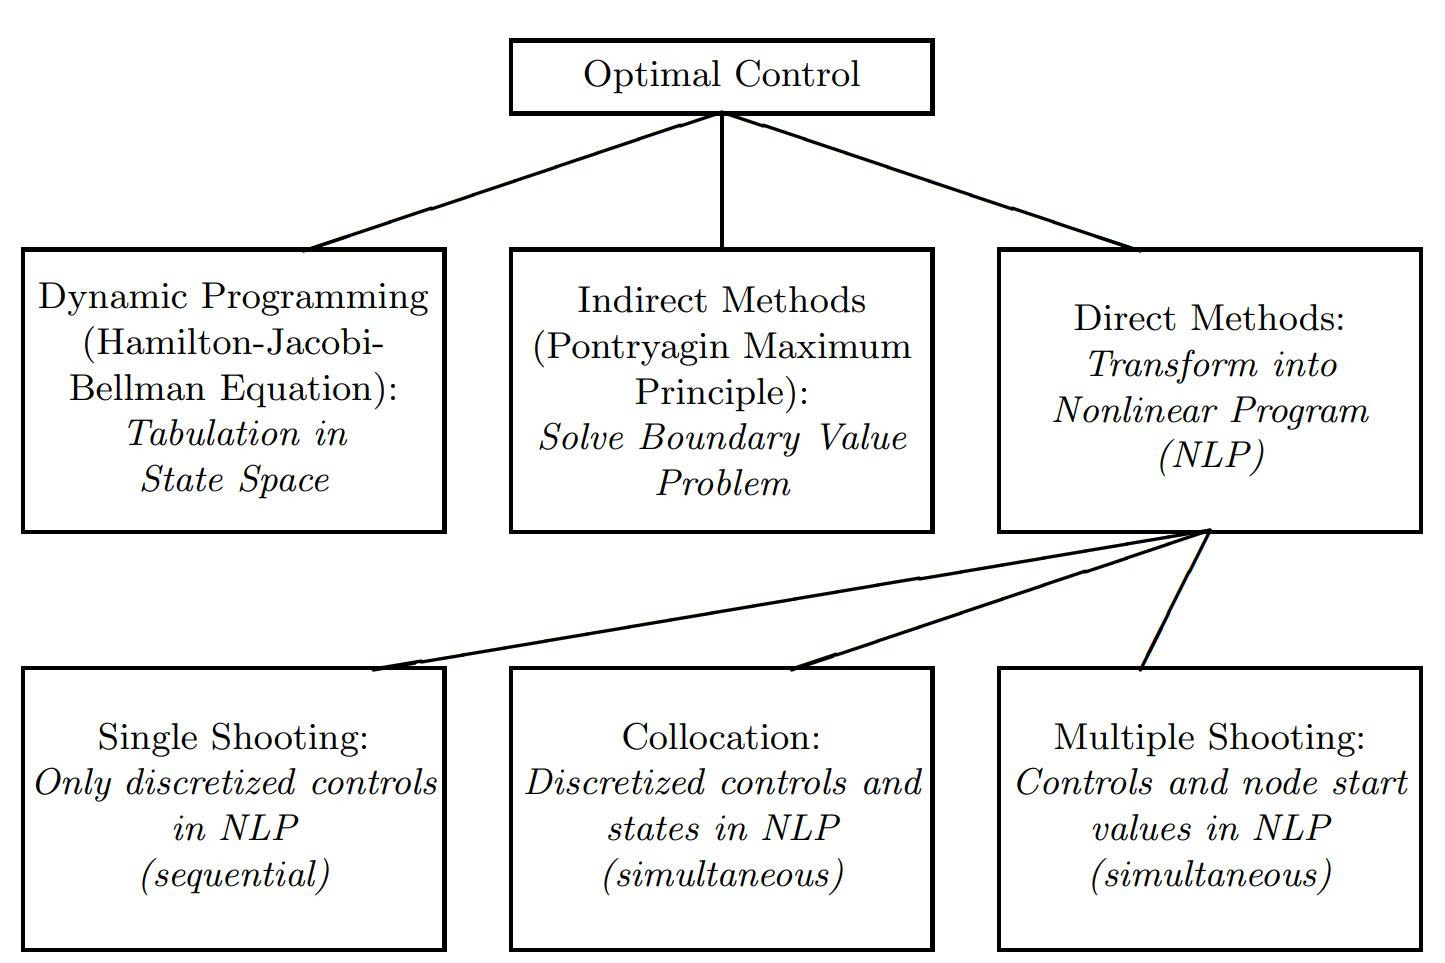
\includegraphics[width=1\textwidth]{theoretical-background/image/numerical-ocp-method.jpg}
    \caption[Một vài phương pháp giải bài toán điều khiển tối ưu]{%
        Ba phương pháp cơ bản để giải quyết các bài toán điều khiển tối ưu, 
        (a) lập trình động, (b) phương pháp gián tiếp và (c) phương pháp trực tiếp ~\cite{DiehlEtAl2006}.}
    \label{fig:ocp_methods}
\end{figure}
Trong các bài toán robotics và motion planning có nhiều ràng buộc, các phương pháp trực tiếp thường là lựa chọn thực dụng hơn. Nguyên nhân là các ràng buộc bất đẳng thức, ràng buộc trạng thái, ràng buộc điều khiển và các thay đổi active set có thể được xử lý trực tiếp trong khung Nonlinear Programming (NLP). Sau khi rời rạc hóa, bài toán OCP được viết về dạng tổng quát
\begin{equation}
    \min_{w} \; a(w)
    \quad
    \text{subject to}
    \quad
    b(w)=0,\qquad c(w)\ge 0,
    \label{eq:nlp_form}
\end{equation}
trong đó $w$ là vector hữu hạn chiều chứa các biến tối ưu, $a(w)$ là hàm mục tiêu hữu hạn chiều, $b(w)=0$ là các ràng buộc đẳng thức, và $c(w)\ge 0$ là các ràng buộc bất đẳng thức.

Từ góc nhìn này, vai trò của một direct method là xây dựng ánh xạ từ bài toán
liên tục \eqref{eq:general_ocp} sang bài toán NLP \eqref{eq:nlp_form}. Sự khác
nhau giữa các direct methods nằm ở cách chúng xử lý quỹ đạo trạng thái. Trong
direct single shooting, trạng thái được sinh ra bằng tích phân tiến từ trạng
thái đầu, nên các biến tối ưu chủ yếu là tham số điều khiển. Trong direct
collocation, cả trạng thái và điều khiển tại các nút hoặc collocation points
đều được đưa vào làm biến tối ưu, còn động lực học được áp bằng các phương
trình đại số xấp xỉ. Direct multiple shooting nằm giữa hai cách nhìn này: nó
chia horizon thành nhiều đoạn, tích phân động lực học cục bộ trên từng đoạn,
đồng thời vẫn giữ các trạng thái đầu đoạn như biến tối ưu độc lập.

Chính vì vậy, multiple shooting có thể được xem là một cách phiên mã OCP vừa
giữ được trực giác mô phỏng của shooting method, vừa tận dụng được ưu điểm của
simultaneous optimization. Đây là bước trung gian quan trọng để đi từ OCP liên
tục theo thời gian đến một NLP hữu hạn chiều có cấu trúc tốt hơn cho solver.
